\documentclass{standalone}
\usepackage[svgnames]{xcolor}
\usepackage{tikz}
\usetikzlibrary{arrows.meta}
\begin{document}
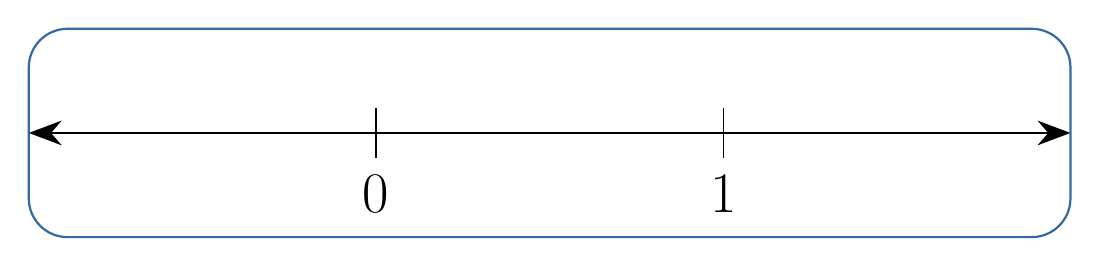
\begin{tikzpicture}[x=1.73611111111111in,y=1.30208333333333in]

\tikzset{
	>={Stealth[scale=1.8]},
	clip even odd rule/.code={\pgfseteorule},
	inverse clip/.style={ clip,insert path=[clip even odd rule]{
		(-1,-0.4) rectangle (2,0.4) }
	}
}
\definecolor{borderblue}{HTML}{356AA0}
\definecolor{fillpurple}{HTML}{A384E5}
\pgfdeclarelayer{background}
\pgfdeclarelayer{foreground}
\pgfsetlayers{background,main,foreground}
\begin{pgfonlayer}{background}
	\fill[white,rounded corners=14pt]
	(-1,-0.4) rectangle (2,0.4);
\end{pgfonlayer}
\huge
\draw[<->,thick] (-1,0) -- (2,0)
node[above left,outer sep=2pt]{\(\)};
\foreach \x in {1,0}{\draw[thin] (\x,9pt) -- (\x,-9pt) node[below]{\(\x\)};}
\draw[borderblue,rounded corners=14pt,thick] (-1,-0.4) rectangle (2,0.4);
\begin{pgfonlayer}{foreground}
\clip[rounded corners=14pt] (-1,-0.4) rectangle (2,0.4);
\end{pgfonlayer}
\begin{pgfonlayer}{background}
\end{pgfonlayer}
\end{tikzpicture}
\end{document}
